\section{Experiments}

To verify that RBN simulation is working as expected,
a RBN is created randomly, initial state set to all zeros, and ran.
The results are visualized in figure \ref{figure:rbn-noperturb}.
We see that the RBN exhibits stable dynamics, and enters into an attractor around $t=15$.
In figure \ref{figure:rbn-perturb} we continiously perturb the RBN with the input stream from the Temporal Parity task visualized in \ref{figure:temporal-parity}.
In the perturbed case, the state trajectory is continiously changed, preventing the RBN from settling into an attractor.
Interestingly enough, there seems to be a visual similarity between the two cases.
Such a pattern is sure to dissapear with a RBN in the chaotic phase.

This erratic pattern of state transitions is then fed into the readout layer,
which is then tasked with finding a linear combination of the RBN states that results in the expected output for the given task.

\begin{figure}
  \subfloat[Unperturbed]{
    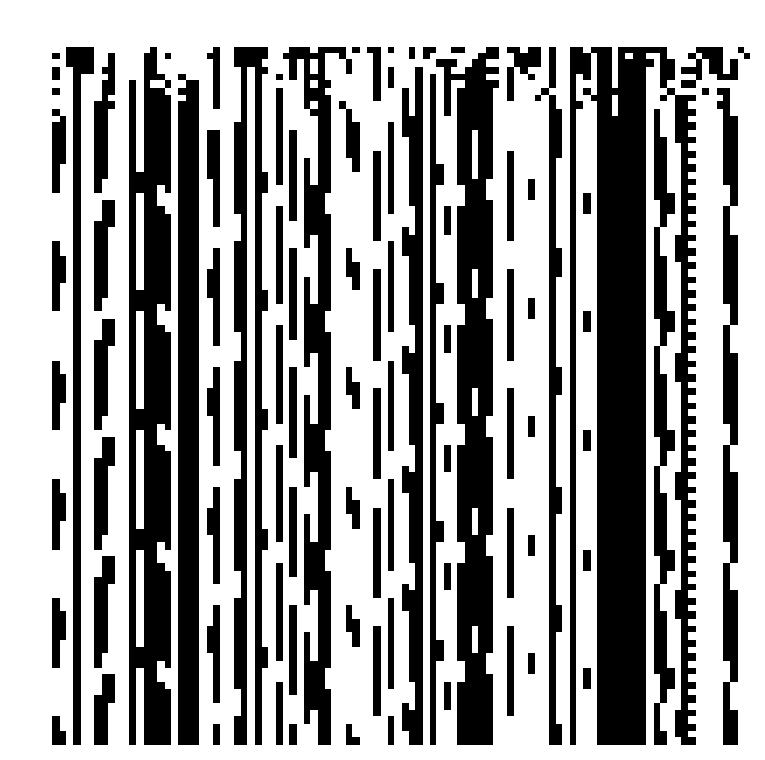
\includegraphics[width=0.5\columnwidth]{method/final-1-noperturb.pdf}
    \label{figure:rbn-noperturb}
  }
  \subfloat[Perturbed]{
    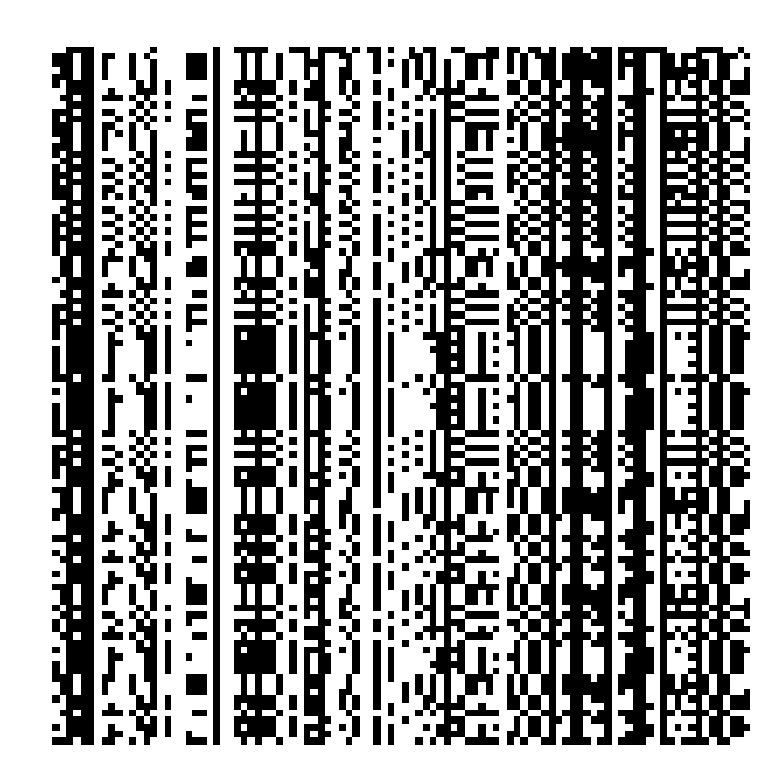
\includegraphics[width=0.5\columnwidth]{method/final-1-perturb.pdf}
    \label{figure:rbn-perturb}
  }
  \caption{
    The same RBN both perturbed and unperturbed.
    Time flows downwards the Y-axis,
    and the current value of each of the nodes in the RBN along the X-axis.
    A cell is white if the value is 1, otherwise black.
    N=100, K=2, P=0.5, L=50, Initial state=0
  }
\end{figure}

\subsection{Reproducing previous experiments}

\subsection{Evolving reservoirs to re-use existing readout layers}

\todo[inline]{Yah this should probably be put somewhere else?}

It seems that for a random sample of reservoirs of a given size and connetivity,
the temporal density task is solveable for a larger $ n $ than the temporal parity one.
The parity task might therefore requires a more specialized network topology to function well.
Due to the seemingly increased complexity of separating the temporal parity task at low $ n $,
it was chosen as the main task in this paper.

